\chapter{Catalan Objects}
Introduce all these things plus concepts/features that will be useful later.
The Catalan numbers are one of the most ubiquitous sequences of numbers in mathematics.  
Named for mathematician Eugene Charles Catalan, the $n\thh$ Catalan number can be succinctly defined as the number of ways of triangulating a convex polygon with $n+2$ sides.  Figure \ref{fig:pentagontriangulations} demonstrates this for the case of $n=3$ The sequence of Catalan numbers for $n \ge 0$ can be defined mathematically as follows:

\begin{align}
    \C_n &= \frac{(2n)!}{n!(n+1)!} =1, 1, 2, 5, 14, 42, 132, \ldots & \text{OEIS} A000108
\end{align}

\begin{figure}
\begin{center}
\begin{tikzpicture}
    \coordinate (a) at (-0,1);
    \coordinate (b) at (0.951,0.309);
    \coordinate (c) at (0.587,-0.809);
    \coordinate (d) at (-0.587,-0.809);
    \coordinate (e) at (-0.951,0.309);


\matrix[column sep=0.8cm,row sep=0.5cm]
{
    \pslice{a/d,a/c} &
    \pslice{b/e,b/d} &
    \pslice{c/a,c/e} &
    \pslice{d/b,d/a} &
    \pslice{e/c,e/b} \\
};
\end{tikzpicture}
\end{center}
    \caption{The $\C_3=5$ triangulations of a polygon with $3+2=5$ sides.}
\label{fig:pentagontriangulations}
\end{figure}
The Catalan numbers can also be expressed through a summation that hints at the recursive structure of many of the Catalan objects.  

\begin{align}
    \C_{n+1} &= \sum_{k=0}^{n}{\C_{k}\C_{n-k}} \textrm{,   }  \C_0=1
\end{align} 

In the case of triangulated polygons, this summation can be derived as follows:

$\C_{n+1}$ is the way of triangulating a convex polygon with $n+3$ sides.  Let $\mathcal{P}_{n+3}$ be a convex $(n+3)$-gon and let $\mathcal{T}$ be a triangulation of $\mathcal{P}_{n+3}$. Fix an edge $e$ in $\mathcal{P}_{n+3}$.  Note that $e$ lies between two vertices of $\mathcal{P}_{n+3}$. $e$ must be in exactly one triaingle in $\mathcal{T}$.  Let $T_{i}$ be the triangle in $\mathcal{T}$ that contains $e$.  $T_{i}$ must have two of its vertices on the two vertices of $e$ and one vertex that is another vertex in $\mathcal{P}_{n+3}$.  There are $n+1$ other vertices of $\mathcal{P}_{n+3}$.  Suppose the third vertex of $T_i$ is $k+1$ vertices clockwise of $e$, where $0\le k \le n$. Drawing $T_i$ divides $\mathcal{P}_{n+3}$ into 3 polygons: $T_i$, a $(k+2)$-gon clockwise of $T_i$, and a $(n-k+2)$-gon counterclockwise of $T_i$. This means that for each possible value of k, there is one way of triangulating $T_i$, $\C_k$ ways of triangulating the polygon clockwise of $T_i$, and $\C_{n-k}$ ways of triangulating the polygon counterclockwise of $T_i$.  Therefore, there are $C_k*C_{n-k}$ ways of triangulating $\mathcal{P}_{n+3}$ for each value of k.  Therefore, there are $\C_{n+1}=\sum_{k=0}^{n}{\C_{k}\C_{n-k}}$ total ways of triangulating $\mathcal{P}_{n+3}$. Figure \ref{fig:recursiveTriangulations} illustrates this process for the case of $n+1=6$.


The Catalan numbers count a remarkable number of interesting and useful combinatorial objects in bijective correspondence with triangulations of $n$-gons. Combinatorial objects counted by the Catalan numbers are referred to as \emph{Catalan objects}.   Richard Stanley's book \emph{Catalan Numbers} gives hundreds of examples of Catalan objects  as well as including a thorough history on the numbers and their study \cite{stanley2015Catalan}. This thesis will focus primarily on three Catalan objects: Dyck words, binary trees, and ordered trees. 


\begin{figure}
    \centering
\begin{center}
\begin{tabular}{ c c c c c c c}
    \octoSliceTable{D} & \octoSliceTable{C}  & \octoSliceTable{B}  & \octoSliceTable{A}  & \octoSliceTable{H}  & \octoSliceTable{G}   \\
    $k=0$ & $k=1$ & $k=2$&$k=3$& $k=4$& $k=5$& \\
    2-gon; 7-gon & 3-gon; 6-gon& 4-gon; 5-gon&5-gon; 4-gon & 6-gon; 3-gon& 7-gon; 2-gon& \\
    $\C_0 *\C_5$ & $\C_1 *\C_4$&$\C_2 *\C_3$ & $\C_3 *\C_2$&$\C_4 *\C_1$ & $\C_5 *\C_0$ \\

    $1 *42$ & $1 * 14$&$2*5$ & $5*2$&$14*1$ & $42*1$ \\
    $42$ & $14$ & $10$ & $10$ & $14$ & $42$
\end{tabular}

\bigskip


$C_6=\sum_{k=0}^5\C_k\C_{n-k}=42 + 14 + 10 + 10 + 14 + 42 = 132$
\end{center}
    \caption{Constructing $\C_6$, the number of ways to triangulate an octagon, from triangulations of smaller sub-polygons.}
    \label{fig:recursiveTriangulations}
\end{figure}
\section{Dyck Words and Paths} \label{sec:Dycks}

The language of binary Dyck words is the set of binary strings that satisfy the following conditions: The string has an equal number of ones and zeroes and each prefix of the string has at least as many ones as zeroes.  The number of distinct Dyck words with $n$ ones and $n$ zeroes is equal to $\C_n$.  Dyck words with $n$ ones and $n$ zeroes are frequently referred to as Dyck words of \emph{order n}.
For example, the $\C_2=2$ Dyck words of order 2 are $1100$ and $1010$.

Two common interpretations of Dyck words are balanced parentheses and paths in the Cartesian plane. If each one in a Dyck word is taken to represent an open parenthesis and each zero a closing parenthesis, the Dyck language becomes the language of balanced parentheses.  Alternatively, the Dyck language can be interpreted as the set of paths in the Cartesian plane using $(1,1)$ (northeast) and $(1,-1)$ (southeast) steps that start at $(0,0)$ and never go below the x axis. In this case, each one in a Dyck word represents a $(1,1)$ step and each zero represents a $(1,-1)$ step.

Figure $\ref{fig:Dycks}$ gives an illustration of each of these interpretations of Dyck words for $n=4$.

\begin{figure}[H]
    \centering
    This figure is temporarily omitted because it is slow
    % \begin{tabularx}{0.55\textwidth}{>{\hsize=0.4\hsize}C >{\hsize=0.2\hsize}C >{\hsize=0.2\hsize}C   }
    %    \thead{Dyck Path} & \thead{Dyck Word} & \thead{Parentheses} \\ \hline 
% \DyckTable[4]{2,2,2,2,0,0,0,0} & 11110000 & (((())))\\
% \DyckTable[3]{2,0,2,2,2,0,0,0} & 10111000 & ()((()))\\
% \DyckTable[3]{2,2,0,2,2,0,0,0} & 11011000 & (()(()))\\
% \DyckTable[3]{2,2,2,0,2,0,0,0} & 11101000 & ((()()))\\
% \DyckTable[2]{2,0,2,2,0,2,0,0} & 10110100 & ()(()())\\
% \DyckTable[2]{2,2,0,2,0,2,0,0} & 11010100 & (()()())\\
% \DyckTable[2]{2,0,2,0,2,2,0,0} & 10101100 & ()()(())\\
% \DyckTable[2]{2,2,0,0,2,2,0,0} & 11001100 & (())(())\\
% \DyckTable[3]{2,2,2,0,0,2,0,0} & 11100100 & ((())())\\
% \DyckTable[2]{2,0,2,2,0,0,2,0} & 10110010 & ()(())()\\
% \DyckTable[2]{2,2,0,2,0,0,2,0} & 11010010 & (()())()\\
% \DyckTable[1]{2,0,2,0,2,0,2,0} & 10101010 & ()()()()\\
% \DyckTable[2]{2,2,0,0,2,0,2,0} & 11001010 & (())()()\\
% \DyckTable[3]{2,2,2,0,0,0,2,0} & 11100010 & ((()))()\\
    % \end{tabularx}
    \caption{The $\C_4=14$ Dyck words of order 4}
    \label{fig:Dycks}
\end{figure}

%TODO: PATHS
% In addition to balanced parentheses, Dyck words of length $2n$ are also in bijective correspondence with extended binary trees with $n$ internal nodes. 
% Given an extended binary tree $B$ with n internal nodes, a Dyck word can be obtained by traversing B in preorder and recording each internal node as a $1$ and each leaf with a $0$, ignoring the final leaf of the tree.

% \begin{figure}
%     \centering
%     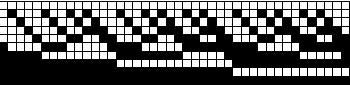
\includegraphics[width=.8\textwidth]{CD5.pdf}
%     \caption{The $\C_5=42$ Dyck words of order 5}
%     \label{fig:dyck5}
% \end{figure}

% TODO

% \section{Grid Paths}
\section{Binary Trees}

Binary trees are fundamental objects in computer science, and are commonly used for searching, sorting, and storing data hierarchically. A binary tree can be defined recursively as follows: The empty set $\phi$ is a binary tree. Otherwise a binary tree has a root vertex, a left subtree, and a right subtree, where each subtree is also a binary tree. A closely related object is an \emph{extended binary tree}, which is a binary tree for which every non-leaf node has exactly two children.  

Binary trees and extended binary trees are both counted by the Catalan numbers: $\C_n$ is the number of binary trees with $n$ nodes and the number of extneded binary trees with $n$ internal nodes.  
A binary tree $b$ with n nodes can be constructed from an extended binary tree $e$ with n internal nodes by removing all leaves from the extended binary tree, leaving the $n$ internal nodes as the only remaining nodes.

This process can be reversed to construct an extended binary tree with n internal nodes from a binary tree with n nodes. Given a binary tree $b$ with n nodes, add two leaf children to every leaf in $b$ and add one leaf child to every node in $b$ with one child. Following these steps, every node originally in $b$ is now an internal node, and therefore the constructed tree is an extended binary tree with n internal nodes.

\section{Ordered Trees}

An ordered tree is a tree for which each node can have an unrestricted number of children and the order of a node's children is significant.  An ordered tree can be defined recursively as follows:


An ordered tree is a tuple $(r,C)$ where $r$ is a root node and $C$ is either the empty set $\phi$ or an ordered sequence of children $(P_1\dots P_m)$ where each $P_i$ is an ordered tree.  Because of the designation of $r$ as a root vertex, an ordered tree cannot be empty, unlike a binary tree.

The number of ordered trees with $n+1$ nodes is equal to $\C_n$.

\begin{figure}
    \begin{subfigure}[]{\textwidth}
	\centering
\begin{tikzpicture}[every tree node/.style={draw,circle},sibling distance=6, level distance=20]
\tikzset{every tree node/.style={minimum width=1.4em,draw,circle},
         blank/.style={draw=none},
         edge from parent/.style=
         {draw,edge from parent path={(\tikzparentnode) -- (\tikzchildnode)}},
         level distance=1.5cm}
    \Tree [.{} [.{} [.{} \edge[draw=none]; \node[blank]{};\edge[draw=none]; \node[blank]{};] \edge[draw=none]; \node[blank]{};] \edge[draw=none]; \node[blank]{};] 
\end{tikzpicture}
\begin{tikzpicture}[every tree node/.style={draw,circle},sibling distance=6, level distance=20]
\tikzset{every tree node/.style={minimum width=1.4em,draw,circle},
         blank/.style={draw=none},
         edge from parent/.style=
         {draw,edge from parent path={(\tikzparentnode) -- (\tikzchildnode)}},
         level distance=1.5cm}
    \Tree [.{} \edge[draw=none]; \node[blank]{};[.{} [.{} \edge[draw=none]; \node[blank]{};\edge[draw=none]; \node[blank]{};] \edge[draw=none]; \node[blank]{};] ] 
\end{tikzpicture}
\begin{tikzpicture}[every tree node/.style={draw,circle},sibling distance=6, level distance=20]
\tikzset{every tree node/.style={minimum width=1.4em,draw,circle},
         blank/.style={draw=none},
         edge from parent/.style=
         {draw,edge from parent path={(\tikzparentnode) -- (\tikzchildnode)}},
         level distance=1.5cm}
    \Tree [.{} [.{} \edge[draw=none]; \node[blank]{};[.{} \edge[draw=none]; \node[blank]{};\edge[draw=none]; \node[blank]{};] ] \edge[draw=none]; \node[blank]{};] 
\end{tikzpicture}
\begin{tikzpicture}[every tree node/.style={draw,circle},sibling distance=6, level distance=20]
\tikzset{every tree node/.style={minimum width=1.4em,draw,circle},
         blank/.style={draw=none},
         edge from parent/.style=
         {draw,edge from parent path={(\tikzparentnode) -- (\tikzchildnode)}},
         level distance=1.5cm}
    \Tree [.{} \edge[draw=none]; \node[blank]{};[.{} \edge[draw=none]; \node[blank]{};[.{} \edge[draw=none]; \node[blank]{};\edge[draw=none]; \node[blank]{};] ] ] 
\end{tikzpicture}
\begin{tikzpicture}[every tree node/.style={draw,circle},sibling distance=6, level distance=20]
\tikzset{every tree node/.style={minimum width=1.4em,draw,circle},
         blank/.style={draw=none},
         edge from parent/.style=
         {draw,edge from parent path={(\tikzparentnode) -- (\tikzchildnode)}},
         level distance=1.5cm}
    \Tree [.{} [.{} \edge[draw=none]; \node[blank]{};\edge[draw=none]; \node[blank]{};] [.{} \edge[draw=none]; \node[blank]{};\edge[draw=none]; \node[blank]{};] ] 
\end{tikzpicture}

	\caption{The $\C_3=5$ binary trees with 3 nodes}
	\label{fig:binarytrees}
	\label{fig:}
    \end{subfigure}
    \begin{subfigure}[]{\textwidth}
	\centering
\begin{tikzpicture}[every tree node/.style={draw,circle},sibling distance=10pt, level distance=40pt]
\tikzset{minimum width=1.5em,edge from parent/.style={draw, edge from parent path=
    {(\tikzparentnode) -- (\tikzchildnode)}}}
    \Tree [.{} [.{} [.{} [.{} ] ] ] ] 
\end{tikzpicture} \hspace{2.9em}
\begin{tikzpicture}[every tree node/.style={draw,circle},sibling distance=10pt, level distance=40pt]
\tikzset{minimum width=1.5em,edge from parent/.style={draw, edge from parent path=
    {(\tikzparentnode) -- (\tikzchildnode)}}}
    \Tree [.{} [.{} ] [.{} [.{} ] ] ] 
\end{tikzpicture} \hspace{2.9em}
\begin{tikzpicture}[every tree node/.style={draw,circle},sibling distance=10pt, level distance=40pt]
\tikzset{minimum width=1.5em,edge from parent/.style={draw, edge from parent path=
    {(\tikzparentnode) -- (\tikzchildnode)}}}
    \Tree [.{} [.{} [.{} ] [.{} ] ] ] 
\end{tikzpicture} \hspace{2.9em}
\begin{tikzpicture}[every tree node/.style={draw,circle},sibling distance=10pt, level distance=40pt]
\tikzset{minimum width=1.5em,edge from parent/.style={draw, edge from parent path=
    {(\tikzparentnode) -- (\tikzchildnode)}}}
    \Tree [.{} [.{} ] [.{} ] [.{} ] ] 
\end{tikzpicture} \hspace{2.9em}
\begin{tikzpicture}[every tree node/.style={draw,circle},sibling distance=10pt, level distance=40pt]
\tikzset{minimum width=1.5em,edge from parent/.style={draw, edge from parent path=
    {(\tikzparentnode) -- (\tikzchildnode)}}}
    \Tree [.{} [.{} [.{} ] ] [.{} ] ] 
\end{tikzpicture}
	\caption{The $\C_3=5$ ordered trees with $3+1=4$ nodes}
	\label{fig:otrees}
    \end{subfigure}
\end{figure}



\section{Bijections}

Since Dyck Words, binary trees, and ordered trees are all Catalan objects, all three sets of objects are in bijective correspondence with each other.  For convenience, we will use the $\mathbf{D}_n$, $\mathbf{B}_n$, $\mathbf{E}_n$, and $\mathbf{T}_n$ to refer to the set of Dyck words of order $n$, the set of binary trees with $n$ nodes, the set of extended binary trees with $n$ internal nodes, and the set of ordered trees with $n+2$ nodes respectively.  

\subsection{Binary Trees and Dyck Words}

The bijection between extended binary trees and Dyck words is particularly elegant: 
For any $e \in \mathbf{E}_n$, traverse e in preorder.  Record a $1$ for each internal node; record a $0$ for each leaf ignoring the final leaf. The resulting binary sequence is a Dyck word  $D \in \mathbf{D}_n $ corresponding to the extended binary tree $e$.  This process can be reversed to go from $\mathbf{D}_n$ to $\mathbf{E}_n$.

\begin{figure}
    \centering
\begin{tikzpicture}[every tree node/.style={draw,circle},sibling distance=6, level distance=20]
\tikzset{every tree node/.style={minimum width=1.5em,draw,circle},
         blank/.style={draw=none},
         edge from parent/.style=
         {draw,edge from parent path={(\tikzparentnode) -- (\tikzchildnode)}},
         level distance=1.5cm}
    \Tree [.{1} [.{1} [.{1} [.\node[style={rectangle,minimum height=.6cm,minimum width=1cm}]{0}; ][.\node[style={rectangle,minimum height=.6cm,minimum width=1cm}]{0}; ]] [.{1} [.\node[style={rectangle,minimum height=.6cm,minimum width=1cm}]{0}; ][.\node[style={rectangle,minimum height=.6cm,minimum width=1cm}]{0}; ]] ] [.{1} [.{1} [.\node[style={rectangle,minimum height=.6cm,minimum width=1cm}]{0}; ][.\node[style={rectangle,minimum height=.6cm,minimum width=1cm}]{0}; ]] [.\node[style={rectangle,minimum height=.6cm,minimum width=1cm}]{0}; ]] ] 
\end{tikzpicture} \hspace{1em}
\begin{tikzpicture}[every tree node/.style={draw,circle},sibling distance=6, level distance=20]
\tikzset{every tree node/.style={minimum width=1.5em,draw,circle},
         blank/.style={draw=none},
         edge from parent/.style=
         {draw,edge from parent path={(\tikzparentnode) -- (\tikzchildnode)}},
         level distance=1.5cm}
    \Tree [.{} [.{} [.{} \edge[draw=none]; \node[blank]{};\edge[draw=none]; \node[blank]{};] [.{} \edge[draw=none]; \node[blank]{};\edge[draw=none]; \node[blank]{};] ] [.{} [.{} \edge[draw=none]; \node[blank]{};\edge[draw=none]; \node[blank]{};] \edge[draw=none]; \node[blank]{};] ] 
\end{tikzpicture}
    \caption{The extended binary tree (left) and binary tree (right) corresponding to the Dyck word 111001001100 \\
    Note that a preorder traversal of the extended binary tree excluding its final leaf yields 111001001100.
    }
\label{fig:binarytreesbijection}
\end{figure}


\subsection{Ordered Trees and Dyck Words}
The bijection between ordered trees and Dyck words is particularly relevant to this paper's results, as it is central to the loopless ordered tree generation algorithm given in Chapter \ref{chap:otree}.
This algorithm will use the bijection between ordered trees and Dyck words specified in Richard Stanley's \emph{Catalan Objects} \cite{stanley2015Catalan}. Figure \ref{ordered_tree_bijection_illustration} illustrates both directions of the bijection.
The bijection can be formalized as follows:
\footnote{ Stanley's text refers to ordered trees as \emph{plane trees} and Dyck words as \emph{ballot sequences}} 


Given an ordered tree T with $n+1$ nodes: Traverse T in preorder.  Whenever going ``down" an edge, or away from the root, record a 1.  Whenever going ``up" an edge, or towards the root, record a 0.  The resulting binary sequence is a Dyck word D corresponding to the ordered tree T. 

This process can be inverted as follows: 

Let $D=d_1...d_{2n}$ be a Dyck word of order $n$ with $n > 0$. Construct an ordered tree T via the following steps. 

Let T be an ordered tree with root $r$.  Keep track of a current node $c$ and set $c$ equal to the root $r$.

\begin{itemize}
    \item For each $d_i$ such that $1 \le i \le 2n$ 
	\begin{itemize}
	    \item if $d_i=1$, then add a rightmost child $ch$ to $c$'s children; set $c=ch$
	    \item if $d_i=0$, then set $c$ equal to $c$'s parent.
	\end{itemize}
	%TODO: QUESTION: do I need to prove this? It seems like Stanely assumed this was basically obvious 

\end{itemize}

\begin{figure}
    \centering
    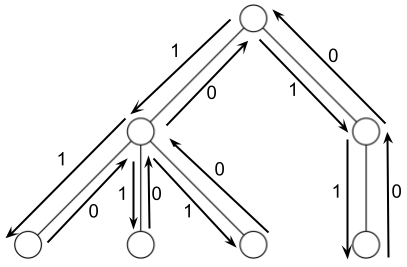
\includegraphics[width=0.5\textwidth]{otreebij.png}
    \caption{An ordered tree with $6+1=7$ nodes corresponding to the order 6 Dyck word $110101001100$.}
    \label{ordered_tree_bijection_illustration}
\end{figure}

\subsubsection{Useful properties of the Ordered Trees $\iff$ Dyck Words bijection}

In addition to the above bijection, we define the following functions relating to ordered trees, Dyck words, and the correspondence between them.

\begin{itemize}
    \item Let $\otree{D}$ and $\dyck{T}$ be functions that convert a Dyck word to an ordered tree and an ordered tree to a Dyck word respectively via the above process.
    \item Let $\depth{t_i}=$ length of path between root and $t_i$. $\depth{root}=0$
    \item Let $\oneindex{D}{i}=$ be the index of the $i\thh{}$ one in D.
\end{itemize}

\bigskip


The following remarks can be derived from the bijection between ordered trees and Dyck words. 


\begin{remark}
    $t_i$ corresponds to the $i$th one in D for $1 \le i \le n$
\end{remark}
\begin{proof}
    Recall the method of constructing an ordered tree from a Dyck word.  Each one in D creates a new node; zeroes in D do not create nodes.  Generating an ordered tree from a Dyck word generates the nodes of the tree in preorder.  Thus, $t_i$ corresponds to the $i$th one in D for $1 \le i \le n$.
\end{proof}

\begin{remark} The difference in depths between nodes $t_i$ and $t_{i-1}$ is equal to one minus the number of zeroes between the $(i-1)^{\underline{st}}$ and $i\thh$ and  ones in $D$


    % TODO: eqref?
\end{remark}
\begin{proof}

    This remark can be stated formally as 

    \begin{equation} \label{eq:depthformula} 
    	\depth{t_i} - \depth{t_{i-1}}=1-(\oneindex{D}{i}-\oneindex{D}{i-1} - 1) 
    \end{equation}
    

    % or equivalently, 

    % \begin{equation} \label{eq:indexformula} 
    % 	\oneindex{D}{i} = \oneindex{D}{i-1} + \depth{t_{i-1}} - \depth{t_i} + 2
    % \end{equation}
    

    Note that $(\oneindex{D}{i}-\oneindex{D}{i-1}-1)$ is equal to the number of zeroes between the $i\thh$ and $(i-1)^{\underline{st}}$ ones in D.  % Therefore, this rule can be informally described as follows:

    % The depth of $t_i$ is the depth of $t_{i-1}$ plus 1 minus the number of zeroes between the $(i-1)\thh$ and $i\thh$ ones in D

    % The number of zeroes between the $i\thh$ and $(i-1)\thh$ ones in $D$ is equal to one plus the depth  $\depth{t_i}$ minus $\depth{t_{i-1}}$

    This follows naturally from the bijection between Dyck words and ordered trees.  Each zero corresponds to a step up in the tree before adding the next child.  

    If there are zero zeroes between the $i\thh$  and $(i-1)^{\underline{st}}$ ones in D, $t_i$ is a child of $t_{i-1}$; $\depth{t_i}=\depth{t_{i-1}}+1$

    If there is one zero between the $i\thh$  and $(i-1)^{\underline{st}}$ ones in D, $t_i$ is a child of $t_{i-1}$'s parent; $\depth{t_i}=\depth{t_{i-1}}+1$.  

    Each subsequent zero between $t_{i-1}$ and $t_i$ decreases $\depth{t_{i}}$ by one.  Thus, the depth of $t_i$ is the depth of $t_{i-1}$ plus 1 minus the number of zeroes between $t_{i-1}$ and $t_{i}$.
\end{proof}
% \bigskip


\begin{remark}A preorder listing of $\depth{t_i} $ for each $ t_i \in T$ can be used to construct a Dyck word. \label{re:construct_dyck}

\end{remark} 
\begin{proof}
    % This follows from Remark \ref{re:depthformula}, as it implies that for any $i,i+1 \le n$, $\oneindex{D}-\oneindex{$ 

    Let $T=t_0,t_1,...t_n$ be a preorder traversal of T.  Note that $t_0$ is the root of $T$

    Construct D as follows: 

    \begin{itemize}
	% \item skip $t_0$
	\item Let $D=\epsilon$ % clear that this is empty string?
	\item For each $t_i$, $1\le i \le n$
	    \begin{itemize}
		\item Append a 1 to $D$
		\item Append $1-\depth{t_{i}}+\depth{t_{i-1}}$ zeroes to D.
	    \end{itemize}
	\item Append $\depth{t_{n}}$ zeroes to D. 
    \end{itemize}
\end{proof} 

% TODO NEW: move to ch 3:, start with binary rule and then get to this.

